\section{Durchführung und Aufbau}
\label{sec:Durchführung}
\subsection{Messprogramm für die Ablenkung im E-Feld}
Zu Beginn wird der Zusammenhang zwischen der Ablenkspannung $U_\text{d}$ und der Verschiebung $D$ für fünf verschiedene Beschleunigungsspannungen $U_\text{B}$ untersucht. Dazu wird die Schaltung aus Abbildung \eqref{fig:Schaltung1} aufgebaut.

\begin{figure}[H]
  \centering
  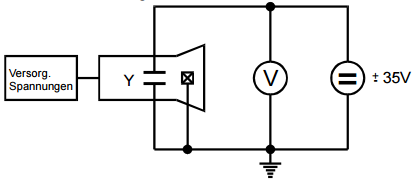
\includegraphics[height=6.5cm]{picture/Schaltung1}
  \caption{Aufbau zur Messung der Abhängigkeit zwischen der Verschiebung und der Ablenkspannung. \cite[5]{V501}}
  \label{fig:Schaltung1}
\end{figure}

Nun wird die Beschleunigungsspannung auf einen Wert zwischen 180V und 500V eingestellt. Daraufhin wird die Ablenkspannung so eingestellt, dass der Leuchtfleck auf der untersten Linie des aufgezeichneten Koordinatensystems zu sehen ist. Die Ablenkspannung wird so verändert das der Leuchtfleck an den ablesbaren Makierungen












\subsection{}
